\section{Zielsetzung}
Ziel des Versuchs ist es, die \textbf{Leerauspannung} und den \textbf{Innenwiderstand} verschiedener
Spannungsquellen zu ermitteln.

\section{Theorie}
Die \textbf{Leerlaufspannung} $U_0$ ist die gemessene Spannung an einer Spannungsquelle, wenn durch diese
kein Strom läuft. Die Spannung $U_0$ wird diekt an der Klemmen der Spannungsquelle abenommen.
Wenn nun ein Verbraucher mit dem Lastwiderstand $R_a$ in den Stromkreis mit eingebaut wird, dann
erhält man die "Klemmspannung" $U_k$, die ebenfalls direkt an den Klemmen der Spannungsquelle abgenommen wird.
Für diese Spannung gilt
\begin{equation*}
  U_k < U_0 \, .
  \label{Gleichung1}
\end{equation*}

 Mit dem zweiten Kirhhoffschen Gesetz

 \begin{equation*}
   \sum_n U_{0_n} = \sum_m R_m \, I_m
   \label{Gleichung2}
 \end{equation*}

 folgt für die dargestellte Situation

 \begin{equation*}
     U_0 = I \, R_i + I \, R_a \ .
     \label{Gleichung3}
 \end{equation*}

 \begin{figure}[h]
   \centering
   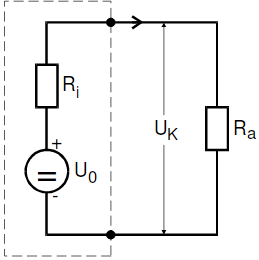
\includegraphics[scale = 0.5]{Bild3.png}
   \caption{Schaltbild einer idealen Spannungsquelle mit Außenwiderstand $R_i$ und
   Lastwiderstand $R_a$ [1]. }
   \label{Abb1}
 \end{figure}
\newpage
 Damit ist auch die Beziehung
 \begin{equation*}
     U_k \approx U_0
 \end{equation*}
 für die Leerlaufspannung gezeigt, da für diesen Fall in \eqref{Gleichung3}
 $I$ vernachlässigbar klein wird. Für diese Betrachtungsweise ist die Spannungsquelle
 eine sogenannte ideale Spannungsquelle mit einem Innenwiderstand von 0 und einem in
 Reihe geschalteten Außenwiderstand $R_i$, der den Innenwiderstand simuliert.

 Bei einem RC-Generator wird durch die Änderung des Belastungsstroms das elektrische
 Verhalten der Quelle festgelegt. In diesem Fall ist der Innenwiderstand eine differentielle
 Größe mit
 \begin{equation}
   R_i = \frac{\symup dU_k}{\symup d I} \ .
   \label{eqn:7}
 \end{equation}

 Für eine Schaltung mit einer Gegenspannung größer als $U_0$ gilt
 \begin{equation}
     U_k = U_0 + R_i \, I
     \label{eqn:8}
 \end{equation}

\section{Durchführung}

Zunächst wird die Klemmspannung der Spannungsquelle gemessen, hierzu wird das Voltmeter direkt an die Spannungsquelle angeschlossen.

Im nächsten Teil des Versuchs wird die ein veränderlicher Widerstand an die Spannungsquelle angeschlossen, wie in Abbildung (???) dargestellt.
Zu messen ist die Spannung $U$ und die Stromstärke $I$ . Es werden 10 Wertepaare für unterschiedliche Widerstände aufgenommen.
Dies wird für 3 Spannungsquellen durchgeführt (Gleich-, Sinus- und Rechteckspannung).
Für die Gleichspannung wird ein Widerstand zwischen 0-50 $\si{\ohm}$ erwendet, für die Sinusspannung ein Widerstand zwischen 20-250 $\si{\ohm}$
und für die Rechteckspannung einen Widerstand zwischen 0,1-5 $\si{\kilo\ohm}$

Im letzten Teil des Experiments wird für die Gleichspannung eine Gegenspannung angeschlossen und erneut die Spannung $U$ und die Stromstärke $I$ gemessen.

\section{Auswertung}
Zur Bestimmung von $U_0$ und $R_\symup{i}$ der drei verschiedenen Spannungsquellen
mittels linearer Regressionen und dem Zusammenhang $U_\symup{k} = U_0 - I R_\symup{i}$
werden jeweils die gemessenen Werte für für die Klemmspannung $U_\symup{k}$ und die Messwerte für
I gegeneinander aufgetragen. Der Steigungswert der Geraden, die durch python ausgegeben
wird, entspricht dabei dem Wert des Innenwiderstandes, der ausgegebene Wert für den y-Achsenabschnitt
liefert den Wert für die Leerlaufspannung.

\subsection{Monozelle ohne und mit Gegenspannung}
Die, wie zuvor beschrieben, ermittelten Werte für die Leerlaufspannung und den Innenwiderstand der Monozelle
ohne Gegenspannung lauten:
\begin{align*}
  R_\symup{i} &= (17,21 \pm 0,22) \Omega \\
  U_0 &= (1,599 \pm 0,011) V
\end{align*}

\begin{table}
  \centering
  \caption{Messwerte zur Bestimmung der Leerlaufspannung und des Innenwiderstands der
  Monozelle}
  \label{tab1}
  \begin{tabular}{c c}
    \toprule
    $I$ / mA & $U$ / V \\
    \midrule
    94  &  0,00   \\
    73  &  0,33   \\
    60  &  0,56   \\
    51  &  0,70   \\
    44  &  0,86   \\
    38  &  0,93   \\
    34  &  1,00   \\
    31  &  1,06   \\
    28  &  1,13   \\
    26  &  1,16   \\
    24  &  1,20   \\
    \bottomrule
  \end{tabular}
\end{table}

\begin{figure}[h!]
  \centering
  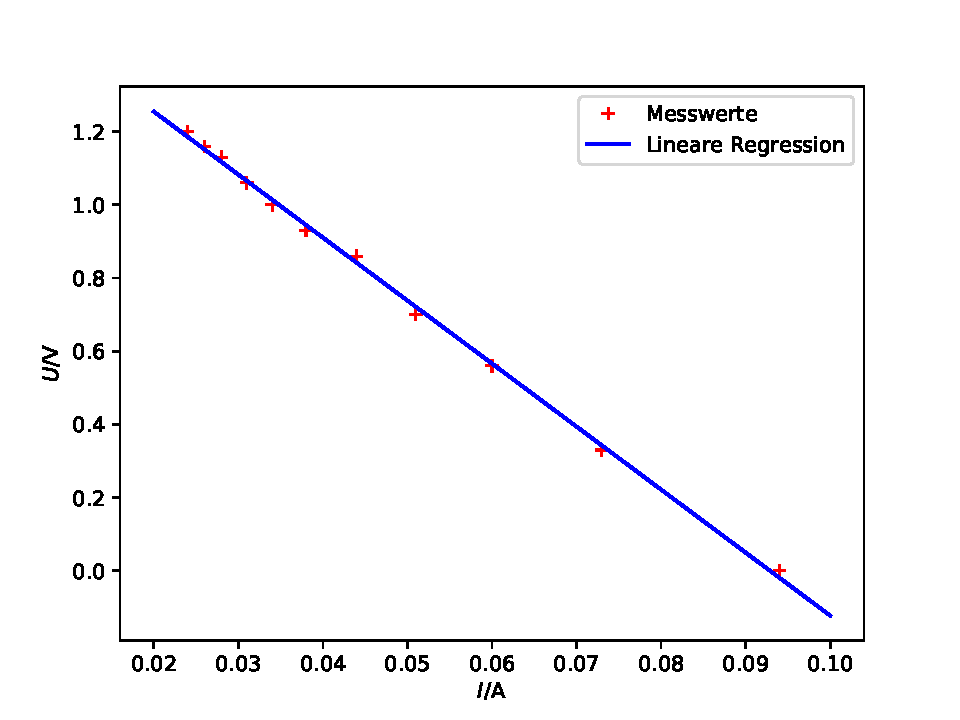
\includegraphics[scale=0.7]{plotA.pdf}
  \caption{Die Messwerte für die Klemmspannung an der Monozelle wurden gegen die gemessene
  Stromstärke aufgetragen.}
  \label{abb4}
\end{figure}
\FloatBarrier

\noindent Wird eine Gegenspannung der Spannung der Monozelle entegegngesetzt, so ergibt sich
aus den genommenen Messwerten \ref{tab2} die in \ref{abb5} zu sehende Regression
und folgende Werte für die Leerlaufspannung und den Innenwiderstand:
\begin{align*}
  R_\symup{i} &= \si{(14,3 \pm 1,3)}{\Omega} \\
  U_0 &= (1,59 \pm 0,08) V
\end{align*}

\begin{table}
  \centering
  \caption{Messwerte für die Klemmspannung und den Strom bei zugeschalteter Gegenspannung}
  \label{tab2}
  \begin{tabular}{c c}
    \toprule
    $I$ / mA & $U$ / V \\
    \midrule
    96  &  3,06  \\
    82  &  2,85  \\
    86  &  2,61  \\
    59  &  2,49  \\
    52  &  2,37  \\
    46  &  2,25  \\
    42  &  2,19  \\
    39  &  2,13  \\
    35  &  2,10  \\
    34  &  2,07  \\
    \bottomrule
  \end{tabular}
\end{table}
\FloatBarrier

\begin{figure}[h!]
  \centering
  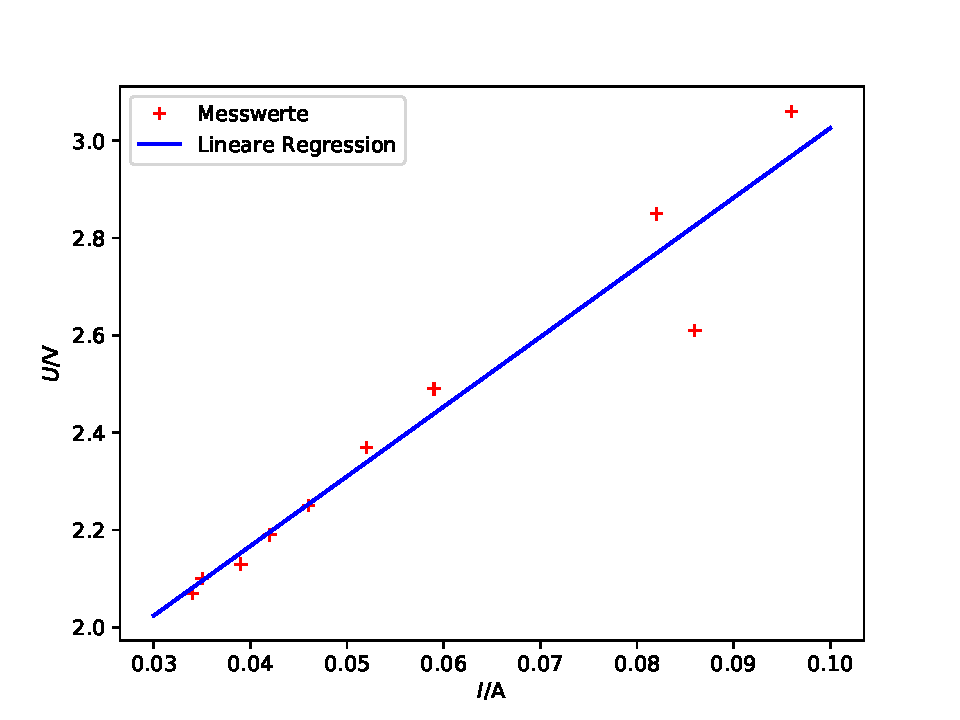
\includegraphics[scale=0.7]{plotD.pdf}
  \caption{lineare Regression zur Bestimmung der Leerlaufspannung und des
  Innenwiderstandes der Monozelle bei zugeschalteter Gegenspannung}
  \label{abb5}
\end{figure}

\noindent Es zeigt sich, dass die Abweichung der experimentell ermittelten Werte
im Bereich der Messungenauigkeit liegen.
\\
\subsection{Rechteck- und Sinusspannung}
Analog zu den beiden bereits durchgeführten Regressionen erfolgt die Ermittlung
der Leerlaufspannung und des Innenwiderstandes einer Rechteck- und einer Sinusspannung.
Zunächst wurde dies für die Rechteckspannung durchgeführt.
In \ref{abb6} ist die lineare Regression zu sehen, die auf Grundlage der Messwerte aus
\ref{tab3} entstanden ist.
Für die Leerlaufspannung und den Innenwiderstand der Rechteckspannung ergeben sich:
\begin{align*}
  R_\symup{i} &= \si{(55,1 \pm 0,6)}{\Omega} \\
  U_0 &= (0,6277 \pm 0,0028) V
\end{align*}

\begin{figure}[h!]
  \centering
  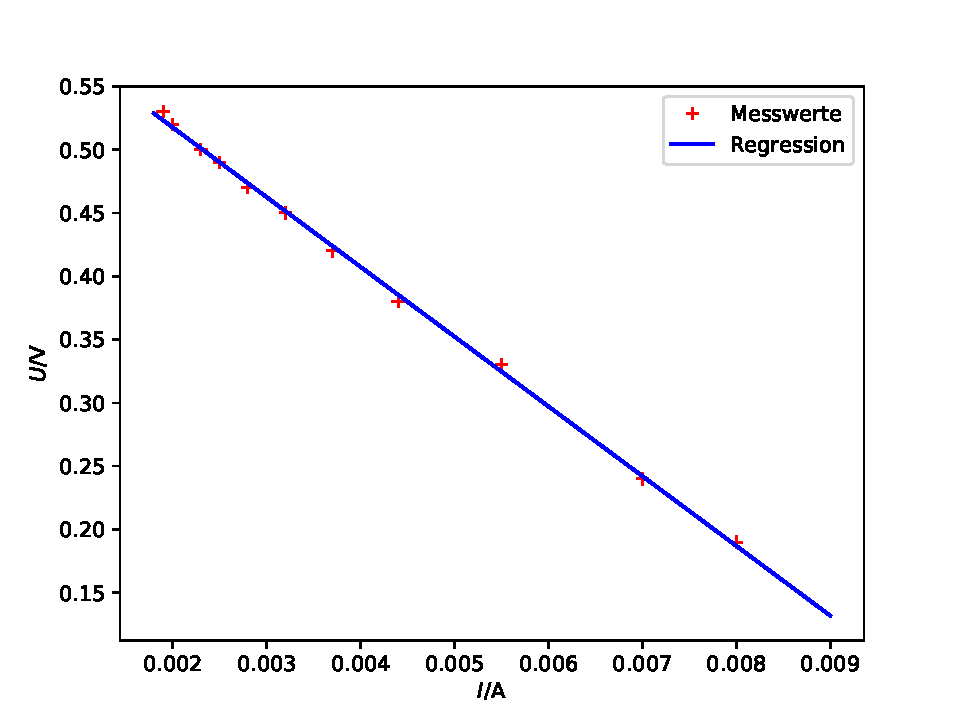
\includegraphics[scale=0.7]{plotB.pdf}
  \caption{Regression zur Ermittlung von $U_0$ und $R_\symup{i}$ einer Rechteckspannung}
  \label{abb6}
\end{figure}
\FloatBarrier

\begin{table}
  \centering
  \caption{Messwerte zur Regression, die in \ref{abb6} dargestellt ist.}
  \label{tab3}
  \begin{tabular}{c c}
    \toprule
    $I$ / mA & $U$ / V \\
    \midrule
    8    &  0,19  \\
    7    &  0,24  \\
    5.5  &  0,33  \\
    4.4  &  0,38  \\
    3.7  &  0,42  \\
    3.2  &  0,45  \\
    2.8  &  0,47  \\
    2.5  &  0,49  \\
    2.3  &  0,50  \\
    2.0  &  0,52  \\
    1.9  &  0,53  \\
    \bottomrule
  \end{tabular}
\end{table}


\noindent Die Leerlaufspannung und der Innenwiderstand des Sinusspannungsgenerators betragen
\begin{align*}
  R_\symup{i} &= \si{(683 \pm 7)}{\Omega} \\
  U_0 &= (1,0774 \pm 0,0034) V .
\end{align*}

Die lineare Regression, die diese Werte lieferte, ist in \ref{abb7} zu sehen. Die
Messwerte, aus denen der Fit erstellt wurde, wiederum in \ref{tab4}.

\begin{figure}
  \centering
  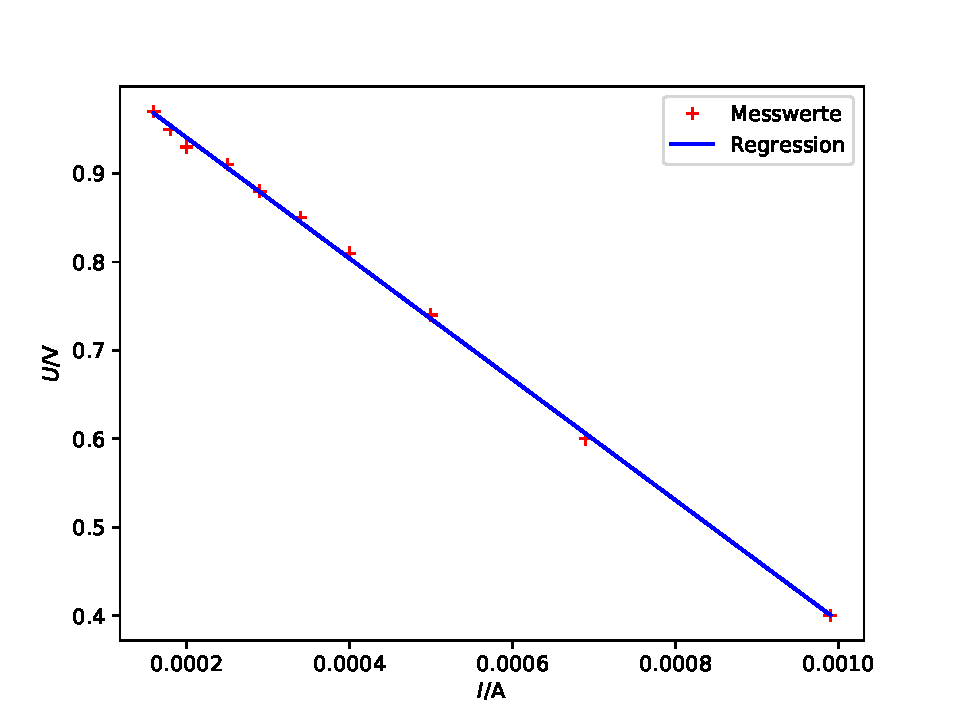
\includegraphics[scale=0.7]{plotC.pdf}
  \caption{Regression zur Ermittlung von $U_0$ und $R_\symup{i}$ einer Sinusspannung}
  \label{abb7}
\end{figure}
\FloatBarrier

\begin{table}
  \centering
  \caption{Messwerte zur Regression, die in \ref{abb7} dargestellt ist.}
  \label{tab4}
  \begin{tabular}{c c}
    \toprule
  $I$ / mA & $U$ / V \\
  \midrule
  0,99  &  0,40  \\
  0,69  &  0,60  \\
  0,50  &  0,74  \\
  0,40  &  0,81  \\
  0,34  &  0,85  \\
  0,29  &  0,88  \\
  0,25  &  0,91  \\
  0,20  &  0,93  \\
  0,18  &  0,95  \\
  0,16  &  0,97  \\
    \bottomrule
  \end{tabular}
\end{table}

\noindent Beide Fehler, der experimentell ermittelten Werte für $R_\symup{i}$ und $U_0$
liegen im Bereich der Messungenauigkeit.


\subsection{Direkte Messung der Leerlaufspannung der Monozelle}
Da das Voltmeter einen endlichen Eingangswiderstand $R_\symup{v}$ von $\SI{10}{\mega\Omega}$ besitzt,
folgt daraus, dass ein systematischer Fehler bei der direkten Messung von $U_0$ auftritt.
$\Delta U$ wird berechnet, indem die Klemmspannung von der Leerlaufspannung abgezogen wird.
Daraus folgt die Formel:
\begin{equation*}
  U_0 - U_\symup{k} = \Delta U = U_\symup{k} \frac{R_\symup{i}}{R_\symup{v}} .
\end{equation*}
Der Fehler für den Spannungsunterschied wird nach Anwendung von Gauß mit folgender Formel berechnet:
\begin{equation*}
  f(R_\symup{i}) =  \frac{U_\symup{k}}{R_\symup{v}} \Delta R_\symup{i}
\end{equation*}
Die gemessene Klemmspannung $U_\symup{k}$ betrug $1,63 V$ , woraus sich zusammen mit dem zuvor experimentell bestimmten
Wert für $R_\symup{i}$ folgender Wert für den Fehler ergibt:
\begin{equation*}
  \Delta U = (16,83 \pm 0,36)\cdot 10^{-7} V
\end{equation*}
Dieser Wert ist so gering, dass die direkte Messung der Leerlaufspannung
an der Monozelle als genau betrachtet werden kann.
\\
Ein im Vergleich zur direkten Messung von $U_0$ signifikanter, systematischer Fehler entstünde,
würde das Voltmeter in der Schaltung hinter das Amperemeter gelegt. Da das hier verwendete Amperemeter
einen sehr großen Widerstand besitzt, um die Strommessung nicht zu beeinflussen, fiele die Spannung
hierüber deutlich ab und die erst danach gemessene Klemmspannung, wäre somit um einiges verringert.

\subsection{Leistungsabfall am Belastungswiderstand}
Die Leistung, die bei der Monozelle im Belastungswiderstand umgesetzt wird, wird ermittelt,
indem die Werte für $U_\symup{k} \cdot I$ gegen $R_\symup{a} = \frac{U_\symup{k}}{I}$ gegeneinander
aufgetragen werden. Die durch die Messdaten beschriebene Kurve wird mit der Theoriekurve für die
Leistung $N (R_\symup{a}) = \frac{U_0^2 R_\symup{a}}{(R_\symup{i} + R_\symup{a})^2}$ verglichen,
um eventuelle systematische Fehler zu ermitteln. Jedoch liegen die Messwerte alle recht nah an der
Theoriekurve, weshalb nicht davon auszugehen ist, dass systematische Fehler gemacht wurden. Messwerte
und Theoriekurve sind in \ref{abb8} zu sehen.

\begin{figure}
  \centering
  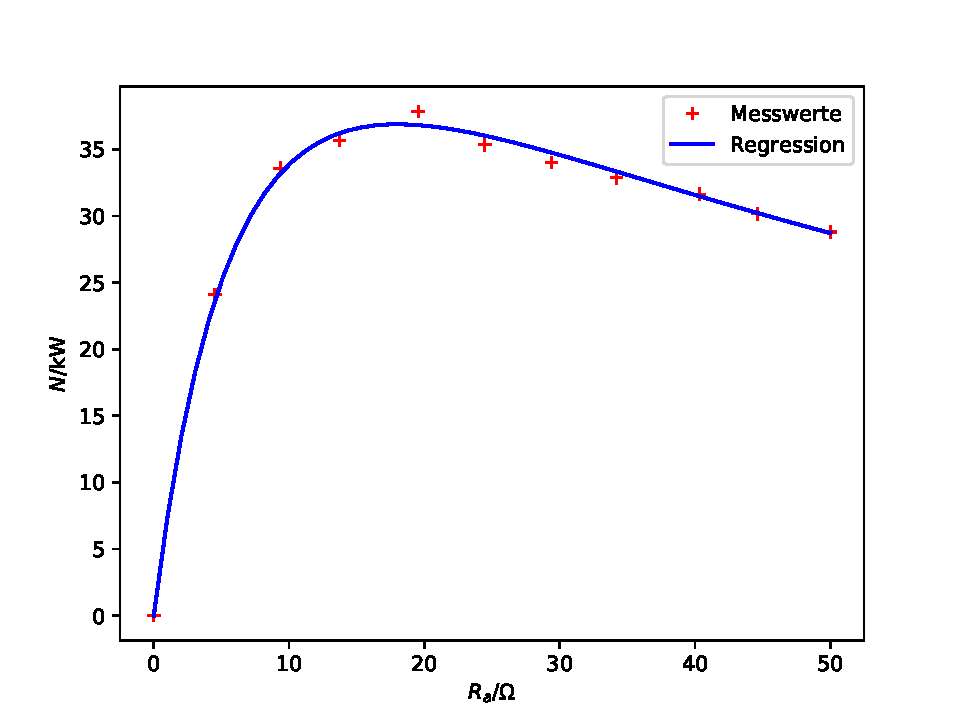
\includegraphics[scale=0.7]{plotN.pdf}
  \caption{Leistungsabfall am Belastungswiderstand.}
  \label{abb8}
\end{figure}

\section{Diskussion}
In den Graphiken ist deutlich zu sehen, dass die Messwerte und deren Fehler stets im Bereich
der Messungenauigkeit lagen. Es ist daher davon auszugehen, dass keine größeren systematischen
Fehler begangen wurden. Ein Vorgehen, das zu ungenaueren Messwerten führen kann, ist das Umstellen
der Skala der Messgeräte für Strom und Spannung. Da darauf jedoch im Vorfeld des Versuchs
hingewiesen wurde, wurde stets darauf geachtet, dass beim Messen kein Umstellen der Skala von
Nöten war. Der vergleichbar große Widerstand für die Sinusspannung im Vergleich zur Rechteckspannung
könnte daran liegen, dass die Amplitude bei den Messungen für die Sinusspannung maximal eingestellt
war, bei der Rechteckspannung war dieser jedoch nur auf halber Stufe.


\section{Literaturverzeichnis}
\begin{enumerate}
  \item Versuchsanleitung Leerlaufspannung und Innenwiderstand von Spannungsquellen: http://129.217.224.2 /HOMEPAGE/MEDPHYS/BACHELOR/AP/SKRIPT/V301.pdf 27.11.2017, 1734uhr)
\end{enumerate}
